
\includegraphics{../../src/includes/figures/vinaya-class-title.w600.png}

\url{https://vinaya-class.github.io}

Read here or download as PDF below for printing.

\begin{itemize}
\tightlist
\item
  \href{./includes/docs/vinaya-class.zip}{vinaya-class.zip} All-in-one
  ZIP archive
\end{itemize}

Individual files:

\begin{itemize}
\tightlist
\item
  \href{./includes/docs/schedule.pdf}{schedule.pdf}
\item
  \href{./includes/docs/sign-up-sheet.pdf}{sign-up-sheet.pdf}
\item
  \href{./includes/docs/class-rules.pdf}{class-rules.pdf}
\item
  \href{./includes/docs/vinaya-class-notes.pdf}{vinaya-class-notes.pdf}
\item
  \href{./includes/docs/vinaya-class-questions-A.pdf}{vinaya-class-questions-A.pdf}
\item
  \href{./includes/docs/vinaya-class-questions-A-answerkey.pdf}{vinaya-class-questions-A-answerkey.pdf}
\item
  \href{./includes/docs/vinaya-class-questions-B.pdf}{vinaya-class-questions-B.pdf}
\item
  \href{./includes/docs/vinaya-class-questions-B-answerkey.pdf}{vinaya-class-questions-B-answerkey.pdf}
\item
  \href{./includes/docs/chanting-refcard.pdf}{chanting-refcard.pdf}
\item
  \href{./includes/docs/chanting-refcard-4on1.pdf}{chanting-refcard-4on1.pdf}
\item
  \href{./includes/docs/vinayakamma-chart.pdf}{vinayakamma-chart.pdf}
\end{itemize}

\section{Schedule}

\href{./includes/docs/schedule.pdf}{schedule.pdf}

\href{./includes/docs/schedule.pdf}{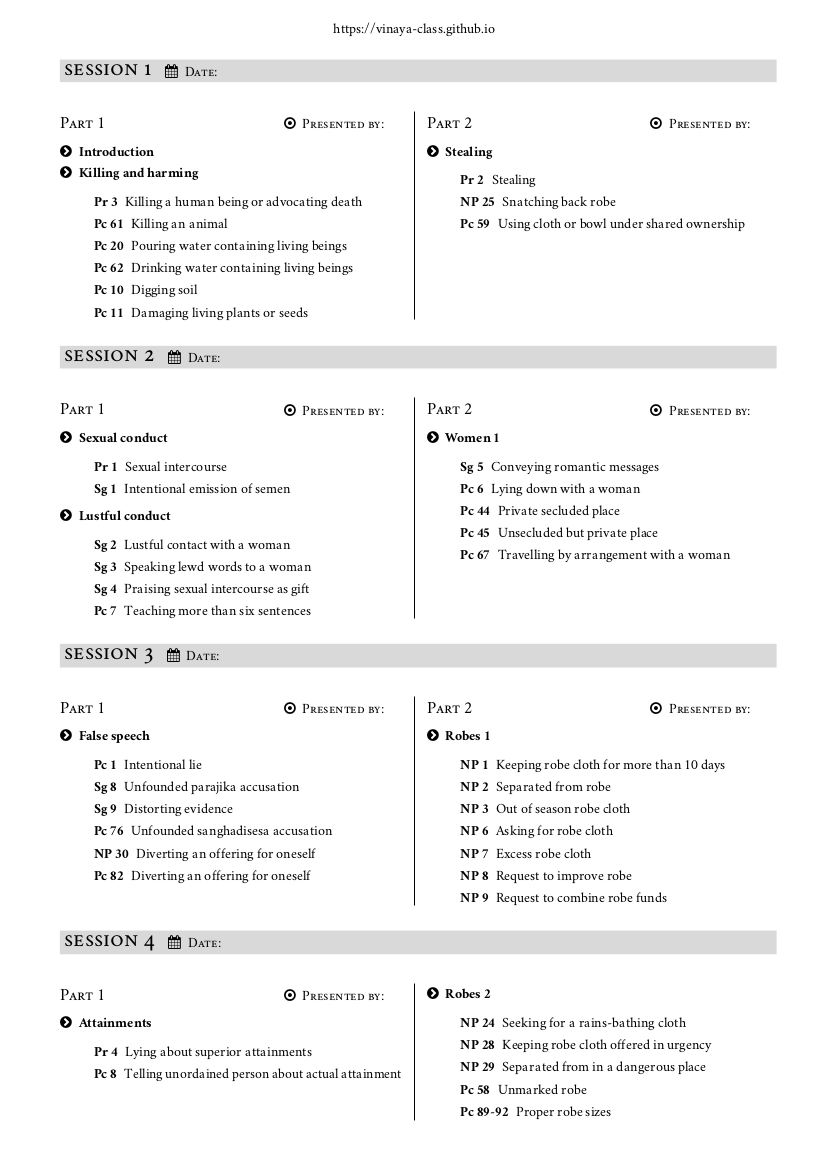
\includegraphics{./includes/docs/schedule-thumb.png}}

\section{Sign-up Sheet}

\href{./includes/docs/sign-up-sheet.pdf}{sign-up-sheet.pdf}

\href{./includes/docs/sign-up-sheet.pdf}{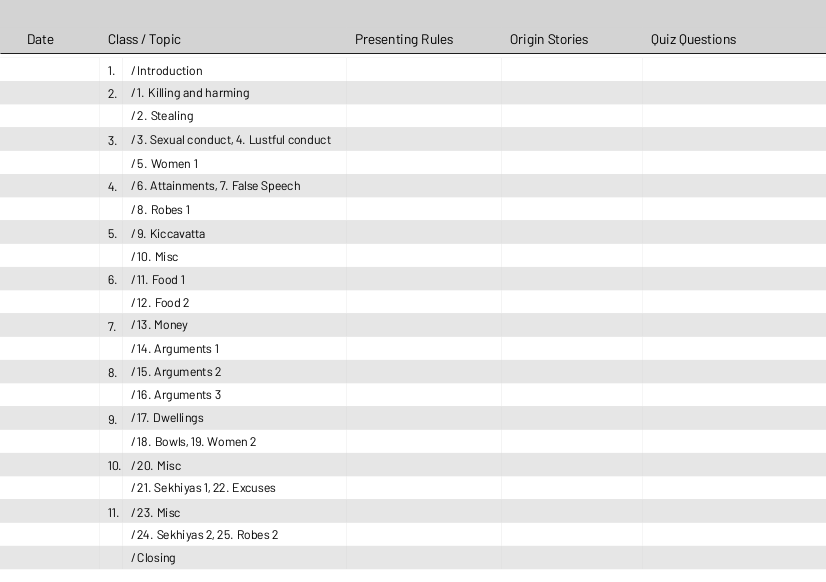
\includegraphics{./includes/docs/sign-up-sheet-thumb.png}}

\section{Class Rules}

\textbf{NOTE:} This is one way to organize the class routine, please
adapt as you see best. One example alternative would be that after
presenting the rules, a large group can be broken up to several smaller
ones for the quiz questions and subsequent discussion, with each
sub-group including at least one experienced /thera/.

\href{./includes/docs/class-rules.pdf}{class-rules.pdf}

\href{./includes/docs/class-rules.pdf}{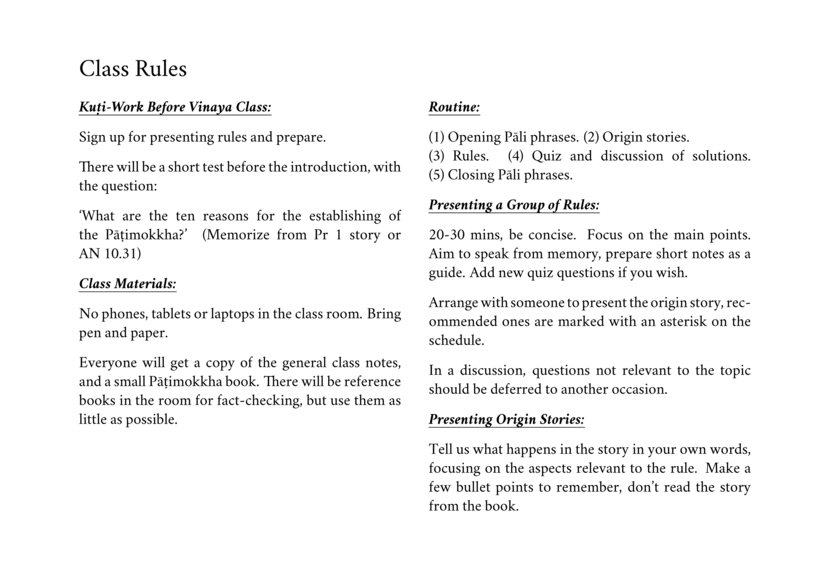
\includegraphics{./includes/docs/class-rules-thumb.png}}

\section{Notes}

\href{./includes/docs/vinaya-class-notes.pdf}{vinaya-class-notes.pdf}

\href{./includes/docs/vinaya-class-notes.pdf}{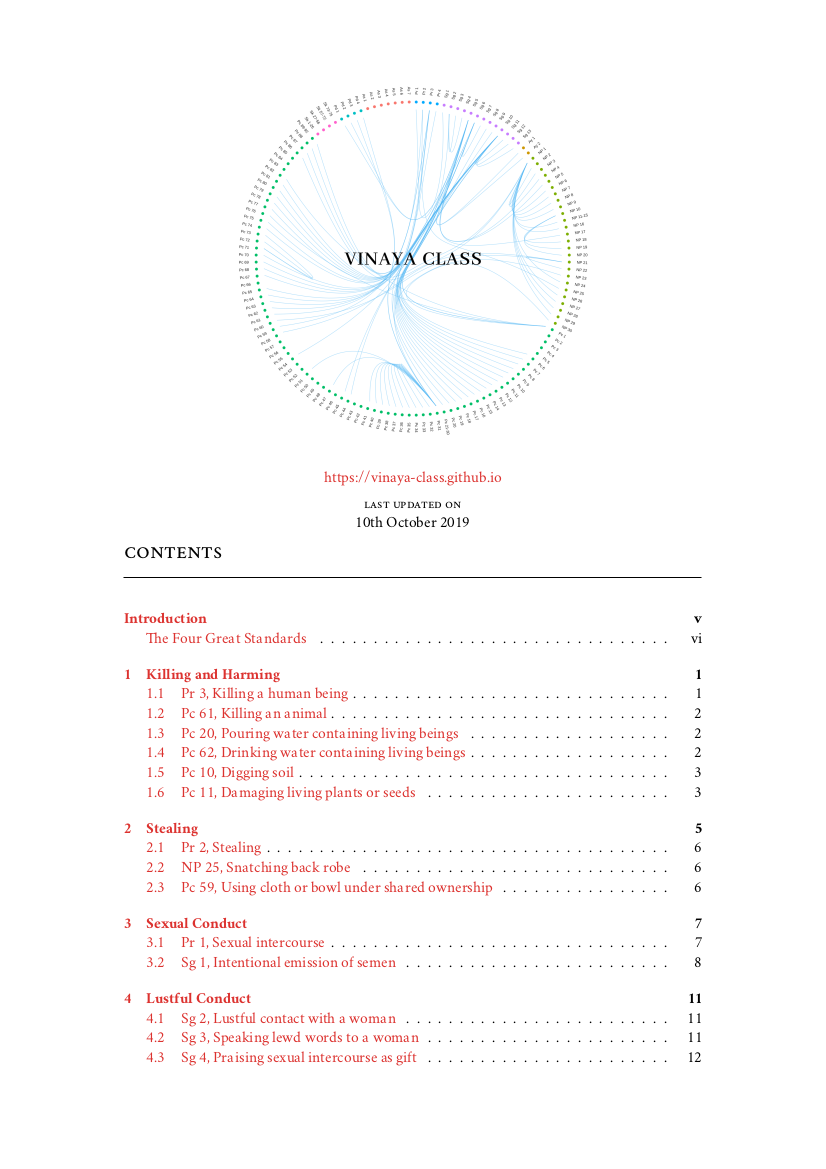
\includegraphics{./includes/docs/vinaya-class-notes-thumb.png}}

\section{Questions}

\textbf{NOTE:} The questions are written to \emph{lean toward} a
particular answer, but they may have different solutions depending on
how one imagined the situation presented. They are intended to be filled
out and reviewed together during the class, discussing the possible
solutions.

\textbf{Series `A'}

\href{./includes/docs/vinaya-class-questions-A.pdf}{vinaya-class-questions-A.pdf}

\href{./includes/docs/vinaya-class-questions-A-answerkey.pdf}{vinaya-class-questions-A-answerkey.pdf}

\textbf{Series `B'}

\href{./includes/docs/vinaya-class-questions-B.pdf}{vinaya-class-questions-B.pdf}

\href{./includes/docs/vinaya-class-questions-B-answerkey.pdf}{vinaya-class-questions-B-answerkey.pdf}

\section{Chanting Refcard}

\href{./includes/docs/chanting-refcard.pdf}{chanting-refcard.pdf}

\href{./includes/docs/chanting-refcard-4on1.pdf}{chanting-refcard-4on1.pdf}

\href{./includes/docs/chanting-refcard-4on1.pdf}{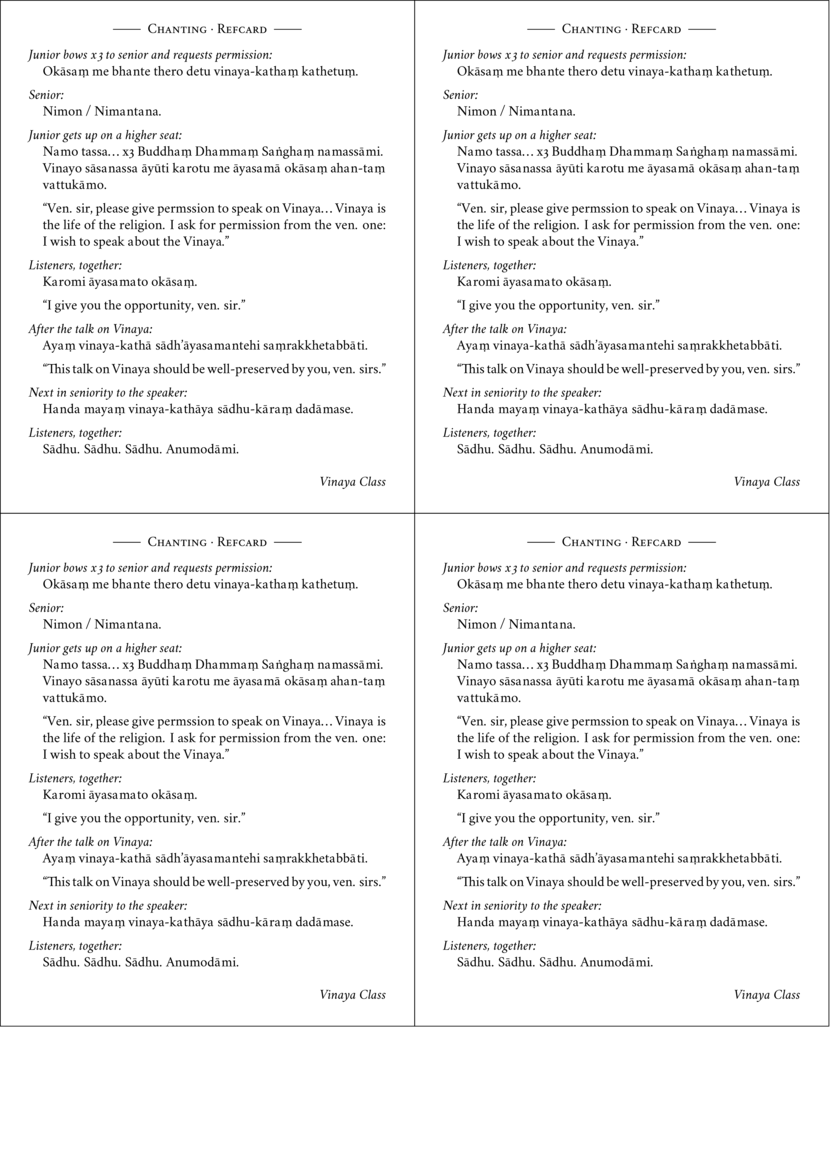
\includegraphics{./includes/docs/chanting-refcard-4on1-thumb.png}}

\section{Vinayakamma}

\href{./includes/docs/vinayakamma-chart.pdf}{vinayakamma-chart.pdf}

\href{./includes/docs/vinayakamma-chart.pdf}{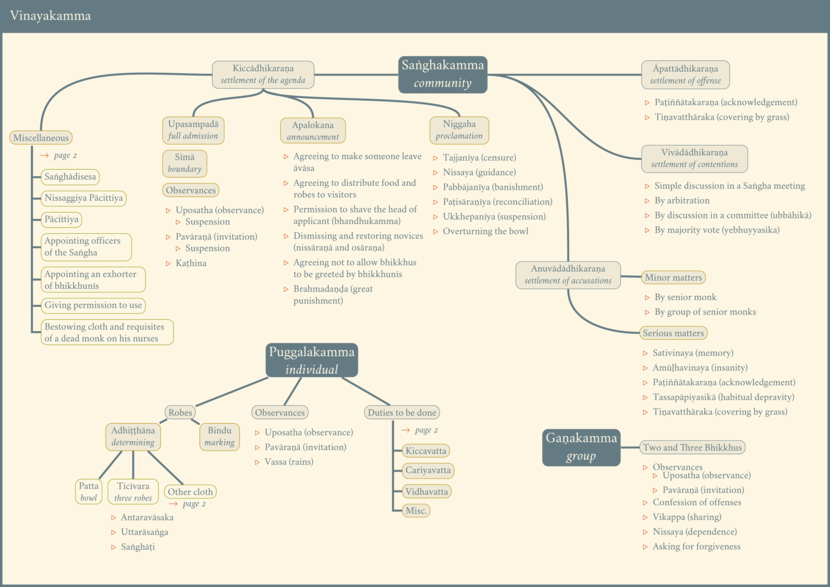
\includegraphics{./includes/docs/vinayakamma-chart-thumb.png}}

